% Generated solely from complete validation analysis.
\subsection{Exploratory validation replication}
Original validation contains 36 independent bases (18 scheduling, 18 workflow), with 2,592 trajectories per model. This analysis was added after the pilot interpretation; validation is not post-amendment held-out confirmation. Table~\ref{tab:validation-repetition} matches the pilot by averaging ordinary synthesis and checklist policies. Each scheduling arm contains 144 decisions from 18 bases. The large pilot benefit does not reproduce in this aggregate; intervals include modest benefits and harms.
\par
\begin{table}[ht]\centering\small\caption{Validation hierarchical scheduling; whole-base 95\% intervals. Differences are repeated minus single.}\label{tab:validation-repetition}
\begin{tabular}{llrrr}\toprule Model & Repetition & Single \% & Repeated \% & Change, pp [95\% CI]\\\midrule
Qwen3-14B & exact & 79.86 & 76.39 & -3.47 [-10.42, 2.78]\\
Qwen3-14B & paraphrase & 79.86 & 78.47 & -1.39 [-5.56, 2.78]\\
Phi-4 & exact & 72.22 & 73.61 & +1.39 [-4.17, 6.25]\\
Phi-4 & paraphrase & 72.22 & 72.92 & +0.69 [-4.17, 4.86]\\
\bottomrule\end{tabular}\end{table}\par
All original comparisons, including scope consolidation, remain in the archived analysis. Policy pooling is explicit; validation and pilot aggregates are not interchangeable. Changes in graph size, parameters, rendering and tie/NONE composition limit a direct causal explanation of the difference between splits.
\begin{figure}[ht]\centering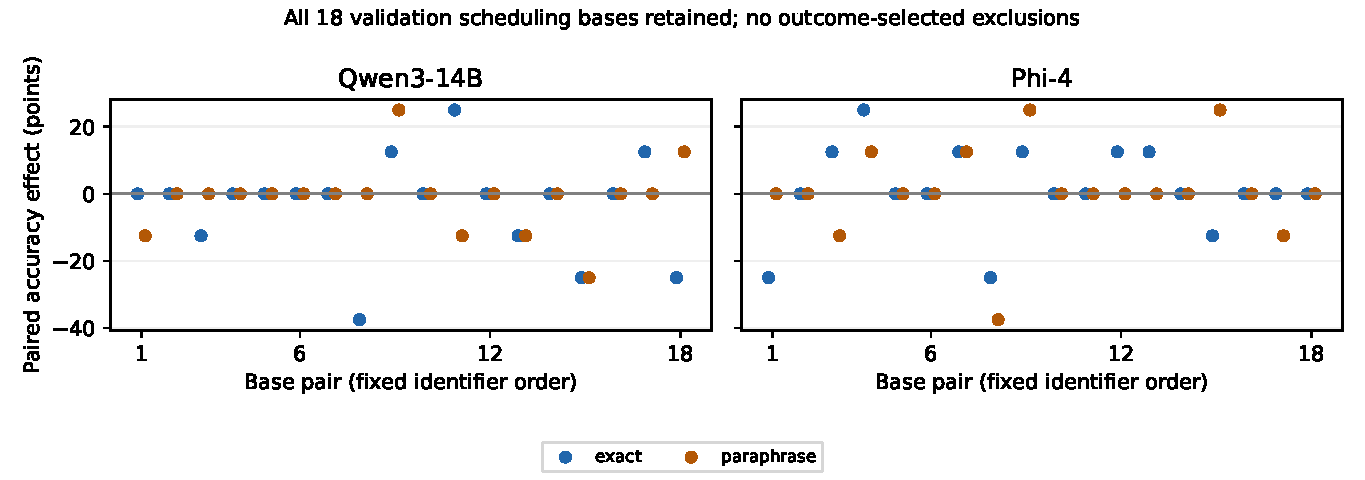
\includegraphics[width=\linewidth]{../results/validation-repetition-v1/figures/base-distribution.pdf}\caption{Validation effects across all 18 scheduling bases; paired worlds, policies and repetitions stay within each base. No outcome-selected exclusions.}\end{figure}
The root-only diagnostic and fresh objective confirmation remain partially or wholly pending. The strict input audit separates contradictory or ill-typed summaries from incomplete consistent information; a correct world answer under inadequate evidence is not evidence of successful integration. The frozen root diagnostic includes selective repetition of each candidate objective and balanced repetition of all objectives, with incoming distinct claims fixed. Its lossless interface is an idealized information-preservation intervention.
